\section{Experiment Definition}

As described in the related work section, \textit{JSCleaner} is able to reduce the size of \acrshort{js} files significantly and, therefore, reduce the \acrshort{plt}. However, it has not been shown that this actually reduces the energy consumption. The \textbf{goal} of our study is: ``\textit{Analyze JSCleaner for the purpose of evaluation with respect to the energy consumption from the point of view of software developers in the context of mobile web pages}". This goal has been established using the GQM method ~\cite{claes2012experimentation}, the steps are presented in Table \ref{tab:gqm}.

\begin{table}[H]
    \caption{GQM}
    \centering
    \begin{tabular}{||c || c||} 
     \hline
     Analyse & JSCleaner \\ 
     \hline
     For the purpose of & evaluating \\
     \hline
     With respect to the & energy consumption \\
     \hline
     From point of view of & developer \\
     \hline
     In the context of & mobile web pages \\
     \hline
    \end{tabular}
\label{tab:gqm}
\end{table}


Following our goal we have identified the main \textbf{research question}: \textbf{[RQ1]} ``\textit{What is the impact of de-cluttering JavaScript code in mobile web pages using \textit{JScleaner} with respect to the energy consumption?}''. We answer this research question by comparing the energy consumption of 500 web pages compared to their de-cluttered version. 

To answer our research question the \textit{energy consumption (joule)} is used as \textbf{metric}. The energy consumption is calculated using the measured \textit{power consumption (joule per second)} times the \textit{\acrshort{plt} (seconds)}.

Figure \ref{fig:gqm} presents a visual representation of the GQM. It hierarchically shows how the goal is obtained using the research question, and how the research question is answered using the metrics.

\begin{figure}[t]
\caption{GQM tree}
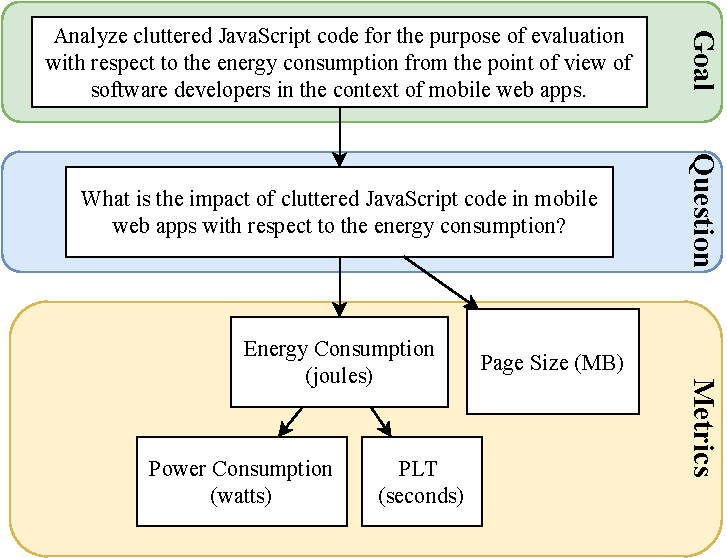
\includegraphics[width=8cm]{reportTemplate/figures/GQM.pdf}
\centering
\label{fig:gqm}
\end{figure}

%\textcolor{red}{Page limit: 2}